\section{设备信息和Kernel特化}
在本章中,我们将探讨使我们的程序更加灵活并因此更加可移植的先进概念。 
这是通过查看与我们的应用程序可能在其上执行的任何系统(和加速器)的功能相匹配的机制
以及我们编写的一系列Kernel和代码来完成的。 
这是一个高级主题,因为我们总是可以简单地“使用默认加速器”并运行我们在其上编写的Kernel,无论它是什么。 
我们了解到,即使在没有加速器的系统上,这也可以工作,
因为 SYCL 保证始终有一个可用的设备可以运行Kernel,即使它是也在运行我们的主机应用程序的 CPU。

当我们超越“使用默认加速器”和通用Kernel时,我们发现可以使用机制来选择要使用的设备,以及创建更特化Kernel的机制。 
我们将在本章中讨论这两种功能。 这两种功能共同使我们能够构建高度适应其执行系统的应用程序。

幸运的是,SYCL 规范的创建者考虑到了这些需求,并为我们提供了接口来让我们解决这个问题。 
SYCL 规范定义了一个设备类,该类封装了可以执行Kernel的设备。 
我们首先涵盖查询设备类别的能力,以便我们的程序能够适应设备的特性和功能。 
我们偶尔可能会选择为不同的设备编写不同的算法。 
在本章后面,我们了解到可以将Aspect应用到Kernel来特化Kernel并让编译器利用它。 
这种特化有助于使Kernel更适合某一类设备,同时可能使其不适合其他设备。 
结合这些概念,我们可以根据自己的意愿或多或少地调整我们的程序。 
这确保我们可以决定在从广泛的可移植性开始的同时,在挤出性能Aspect进行多少投资。

\subsection{是否有 GPU?}
我们中的许多人都会首先通过逻辑来弄清楚“是否存在 GPU?” 告知我们的程序在执行时将做出的选择。 
这就是本章内容的开始。 正如我们将看到的,有更多的信息可以帮助我们使我们的程序变得健壮和高性能。

\begin{remark}
	对程序进行参数化有助于提高正确性、功能可移植性、性能可移植性和面向未来。
\end{remark}

本章深入探讨最重要的查询以及如何在我们的程序中有效地使用它们。 实现无疑提供了我们可以查询的更详细的属性。 
要了解所有可能的查询,我们需要查看最新的 SYCL 规范、特定编译器的文档以及我们可能遇到的任何运行时/驱动程序的文档。

可以使用 get\_info 函数查询特定于设备的属性,包括访问特定于设备的Kernel和Work-Groups属性。

\subsection{细化Kernel代码使其更加规范}
考虑到我们的编码(逐个Kernel)将大致分为以下三类之一是有用的:

\begin{itemize}
	\item \textbf{通用Kernel代码} :在任何地方运行,无需针对特定类别的设备进行调整。

	\item \textbf{设备类型特定的Kernel代码}:在某种类型的设备(例如 GPU、CPU、FPGA)上运行,
	而不是针对设备类型的特定模型进行调整。 这特别有用,因为许多设备类型共享共同的功能,
	因此可以安全地做出一些不适用于为所有设备编写的完全通用代码的假设。

	\item \textbf{调整的特定于设备的Kernel代码}:在一种设备上运行,
	并根据设备的特定参数进行调整——这涵盖了从少量调整到非常详细的优化工作的广泛可能性。
\end{itemize}

\begin{remark}
	作为程序员,我们的工作是确定何时需要不同的设备类型。我们用第14、15、16和17章来阐明这一重要思想。
\end{remark}

最常见的做法是首先关注如何使用通用Kernel的功能正确的实现来工作。 
第 2 章特化讨论了在开始使用Kernel实现时哪些方法最容易调试。 
一旦Kernel开始工作,我们就可以对其进行改进以适应特定设备类型或设备型号的功能。

第 14 章提供了一个在我们深入考虑设备之前首先考虑并行性的思维框架。 
我们对模式(又名算法)的选择决定了我们的代码,而作为程序员,我们的工作就是确定不同设备何时需要不同的模式。 
第 15 章 (GPU)、第 16 章 (CPU) 和第 17 章 (FPGA) 更深入地探讨了区分这些设备类型并促使选择使用模式的品质。 
当最佳方法(模式选择)因不同设备类型而异时,正是这些品质促使我们考虑编写不同版本的Kernel。

当我们为特定类型的设备(例如特定的 CPU、GPU、FPGA 等)编写Kernel时,
将其适应特定供应商甚至此类设备的型号是合乎逻辑的。 
良好的编码风格是根据功能参数化代码(例如,从设备查询中找到的项目大小支持)。

我们应该编写代码来查询描述设备实际功能的参数,而不是其营销信息; 
查询设备的型号并对其做出反应是不好的编程习惯——这样的代码不太可移植,因为它不适合未来。

通常为我们想要支持的每种设备类型编写不同的Kernel(GPU 版本的Kernel和 FPGA 版本的Kernel,也许还有通用版本的Kernel)。 
当我们变得更具体时,为了支持特定的设备供应商甚至设备模型,当我们可以参数化Kernel而不是复制它时,我们可能会受益。 
我们可以自由地选择我们认为合适的任何一个。 因太多参数调整而混乱的代码可能难以阅读或在运行时负担过重。 
然而,参数可以整齐地适合单个版本的Kernel是很常见的。

\begin{remark}
	当算法大致相同但已针对特定设备的功能进行调整时,参数化最有意义。
	当使用完全不同的方法、模式或算法时,编写不同的Kernel要干净得多。
\end{remark}

\subsection{如何枚举设备和功能}
第 2 章列举并解释了选择执行设备的五种方法。 
本质上,方法\#1 是最不规范的,在某个地方运行它,我们发展到最具规范性的方法\#5,
它考虑在一系列设备中的一个相当精确的设备模型上执行。 介于两者之间的列举方法兼具灵活性和规范性。 
图 12-1、图 12-2 和图 12-4 帮助说明我们如何选择设备。

\begin{figure}[H]
	\centering
	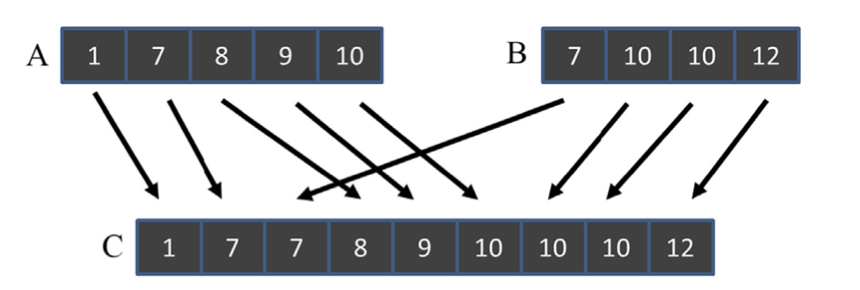
\includegraphics[width=0.9\textwidth]{figs/F12.1.png}
	\caption{\textit{默认情况下已为我们分配的设备 }}
\end{figure}

图 12-1 显示,即使我们允许实现为我们选择默认设备(第 2 章中的方法\#1),
我们仍然可以查询有关所选设备的信息。

\begin{figure}[H]
	\centering
	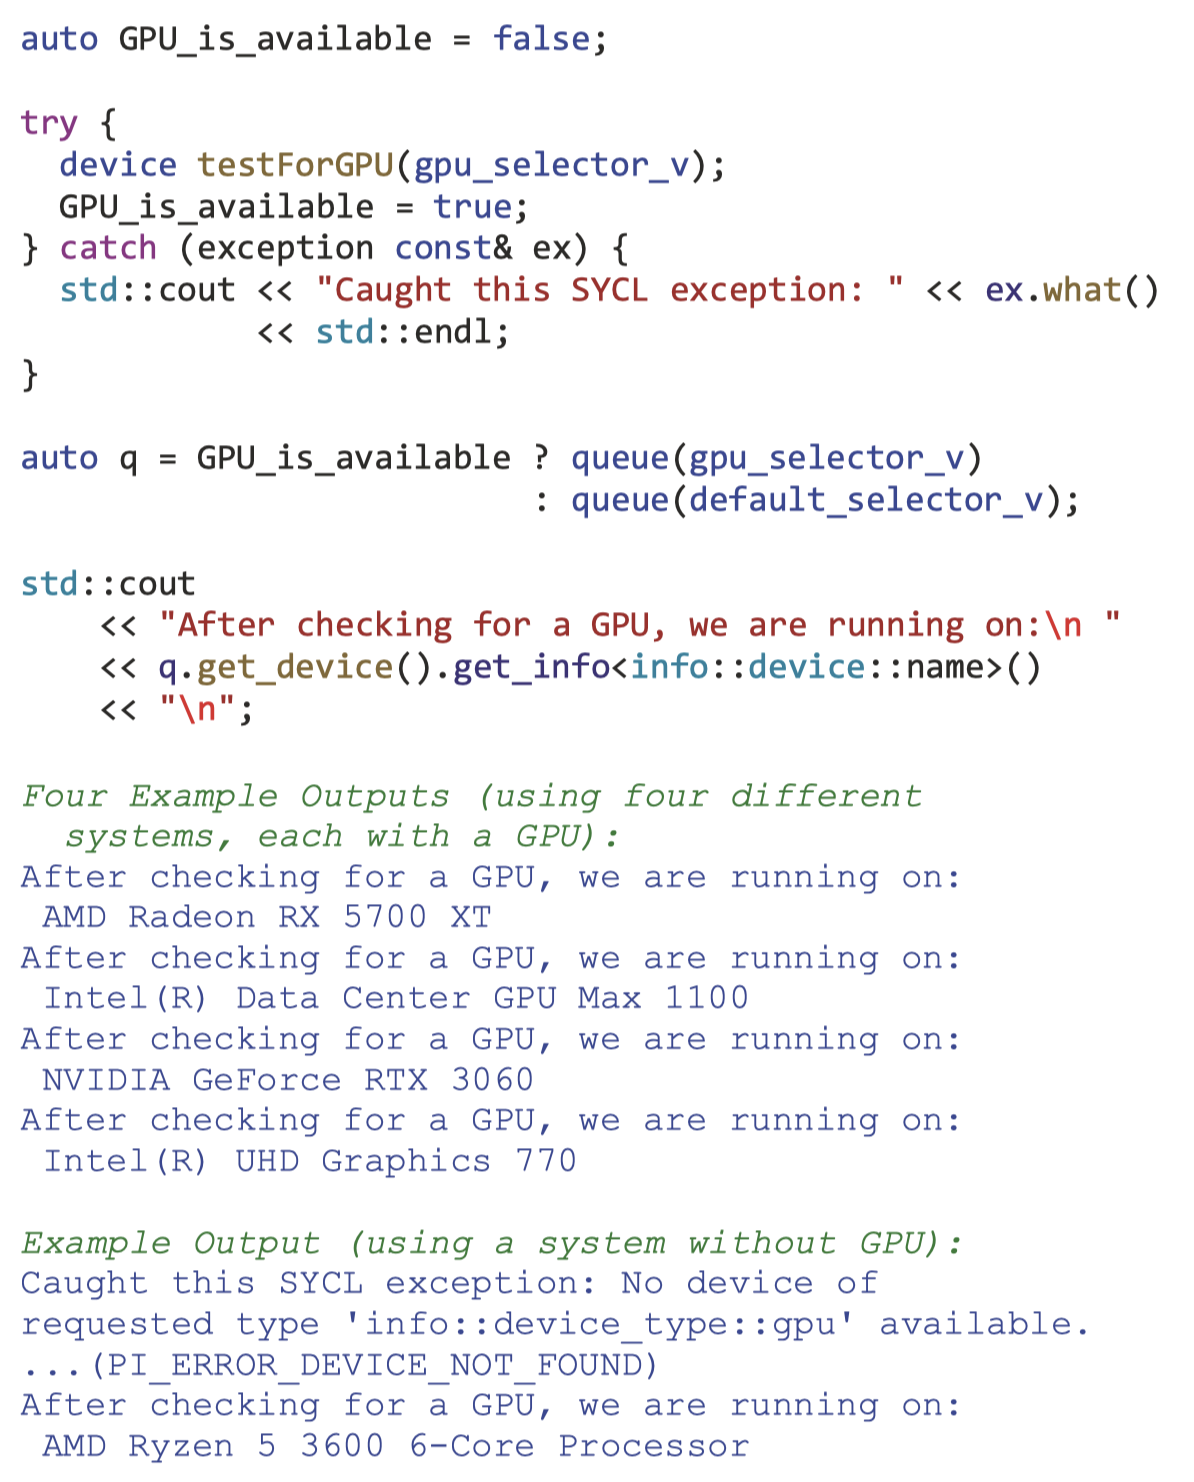
\includegraphics[width=0.9\textwidth]{figs/F12.2.png}
	\caption{\textit{如果可能,请使用 try-catch 选择 GPU 设备,如果没有,请使用默认设备 }}
\end{figure}

图 12-2 显示了我们如何尝试使用特定设备(在本例中为 GPU)设置队列,但如果没有可用的 GPU,则显式回退到默认设备。 
这让我们能够在一定程度上控制设备的选择,只要有可用的 GPU,我们就会优先选择 GPU。 
我们知道至少有一个设备始终保证存在,因此我们的Kernel始终可以在正确配置的系统中运行。 
当没有 GPU 时,许多系统会默认使用 CPU 设备,但这并不能保证。 
同样,如果我们显式请求一个 CPU 设备,则不能保证存在这样的设备(但我们保证某个设备将存在)。

不建议使用图12-2所示的方案。 除了看起来有点可怕和容易出错之外,如果运行时可以选择 GPU,
图 12-2 并不能让我们控制选择哪个 GPU。 尽管既有指导意义又实用,但还有更好的方法。 
建议我们编写自定义设备选择器,如下一个代码示例(图 12-4)所示。

有关设备的查询依赖于已安装的软件(特殊的用户级驱动程序)来响应有关设备的信息。 
SYCL 依赖于此,就像操作系统需要驱动程序来访问硬件一样,仅将硬件安装在计算机中是不够的。

\subsubsection{Aspect}
\begin{figure}[H]
	\centering
	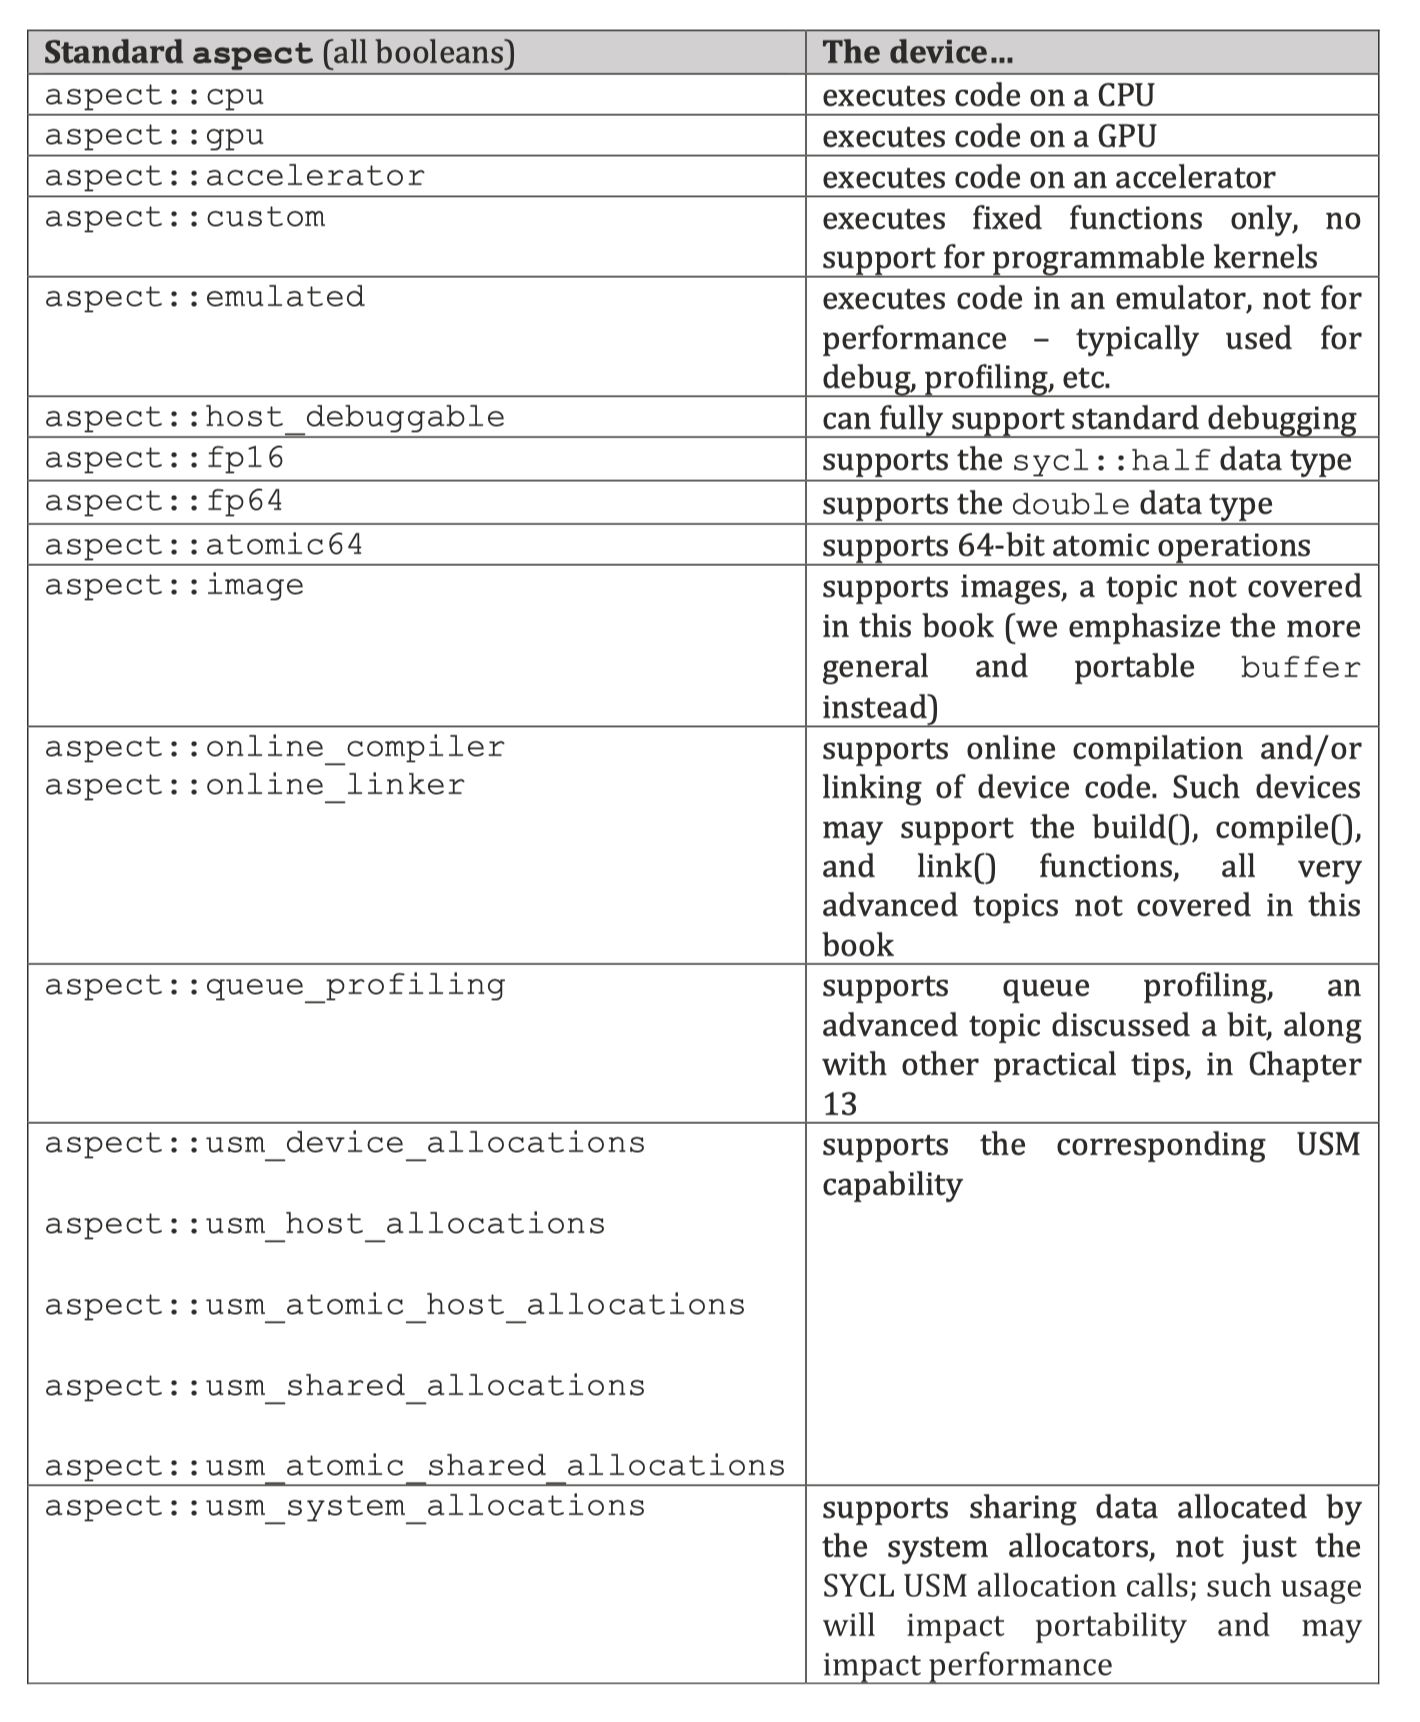
\includegraphics[width=0.9\textwidth]{figs/F12.3.png}
	\caption{\textit{SYCL 标准定义的Aspect(实现可以添加更多) }}
\end{figure}

SYCL 标准有一个设备Aspect的小列表,可用于了解设备的功能、控制我们选择使用哪些设备以及控制我们向设备提交哪些Kernel。 
在本章的最后,我们将讨论“Kernel特化”和Kernel模板化。 现在,我们将列举这些Aspect以及如何在设备查询和选择中使用它们。 
图 12-3 列出了 SYCL 标准定义的Aspect,可用于每个使用 SYCL 的 C++ 程序。 
Aspect是布尔值——设备要么有Aspect,要么没有Aspect。 
前四个(cpu/gpu/加速器/自定义)是互斥的,因为设备类型被 SYCL 2020 定义为枚举。
包括aspect::fp16、aspect::fp64 和aspect::atomic64 在内的功能是“可选功能”,
因此 它们可能不受所有设备的支持 - 对这些设备的测试对于强大的应用程序尤其重要。

\subsubsection{自定义设备选择器}
\begin{figure}[H]
	\centering
	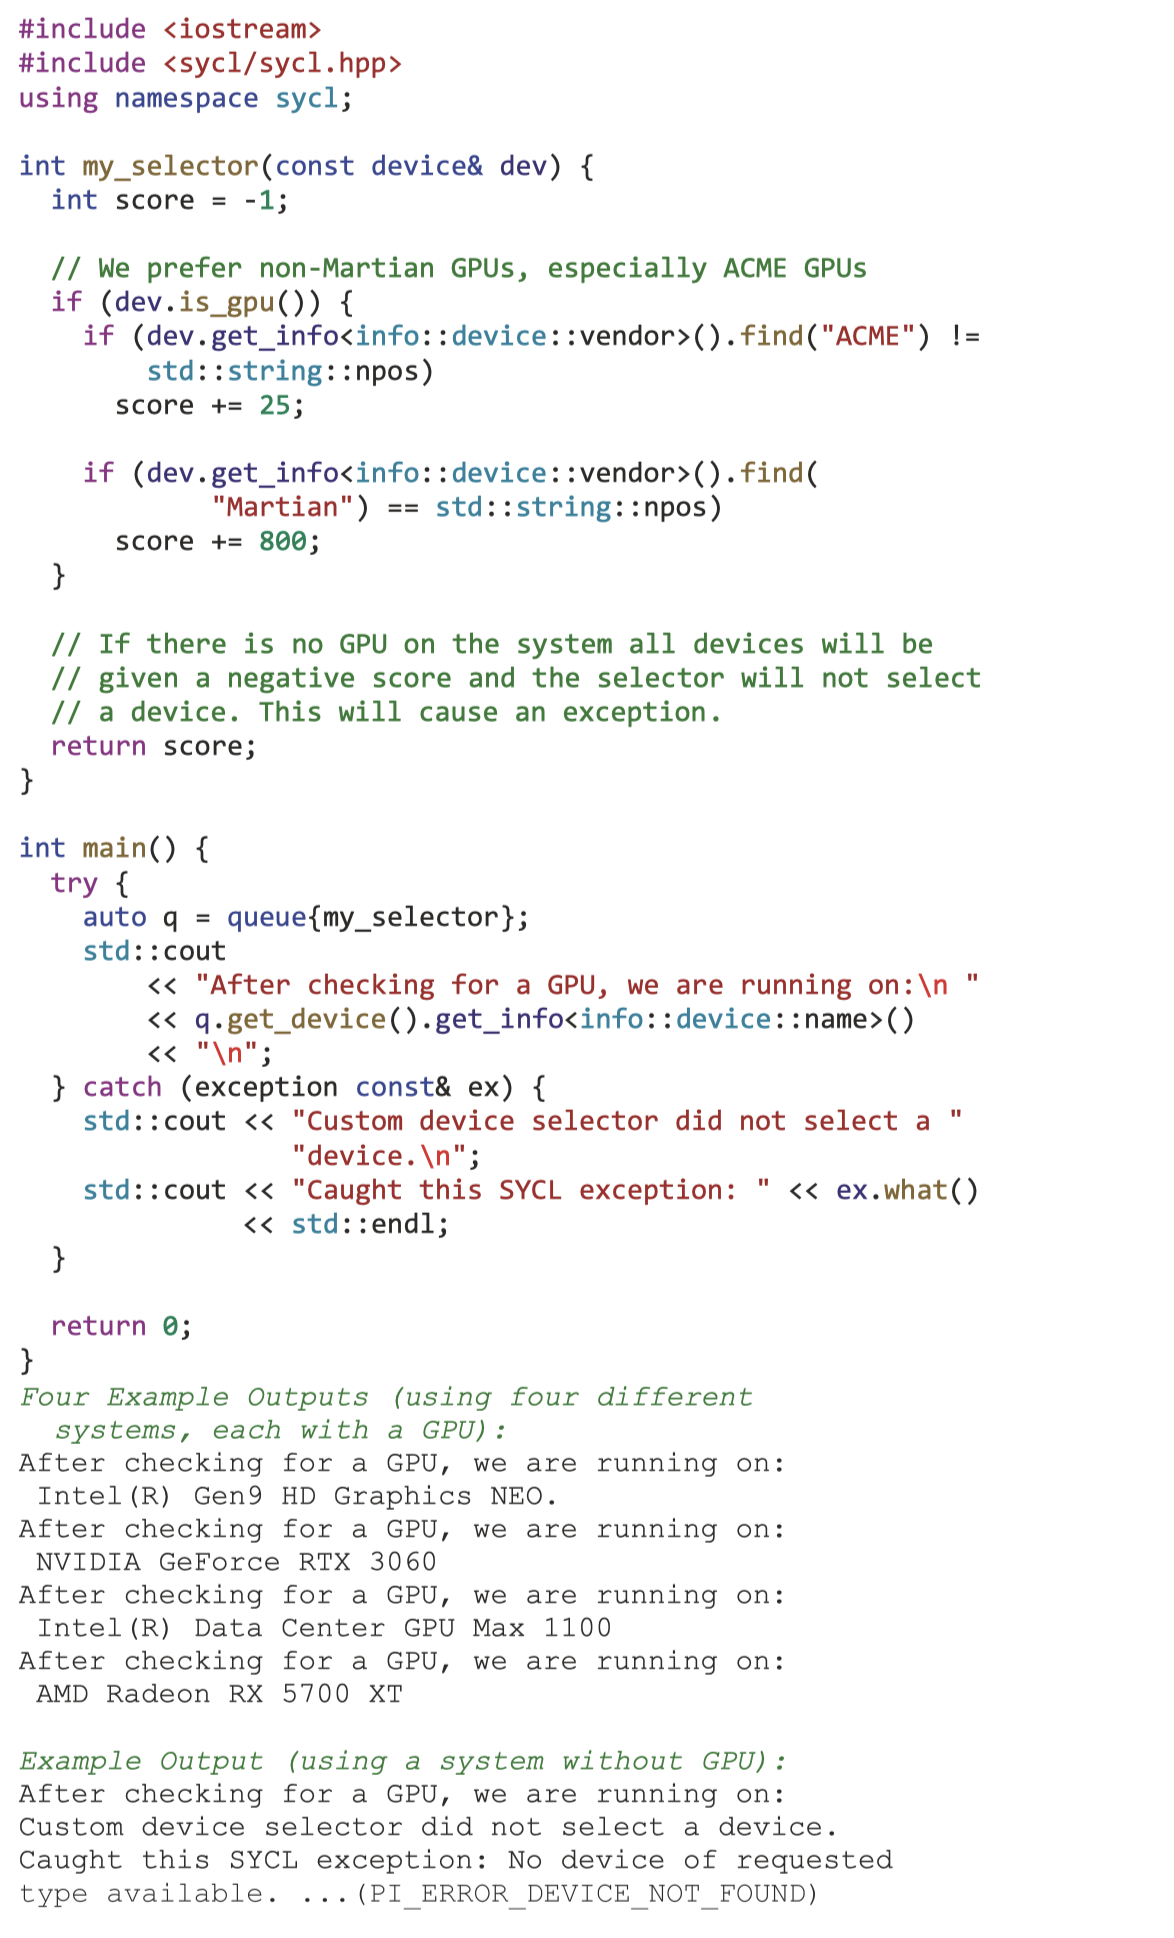
\includegraphics[width=0.9\textwidth]{figs/F12.4.png}
	\caption{\textit{自定义设备选择器 — 我们的首选解决方案 }}
\end{figure}

图 12-4 使用自定义设备选择器。 自定义设备选择器首先在第 2 章中作为 Method\#5 讨论,
用于选择代码运行的位置(图 2-16)。 自定义设备选择器评估应用程序可用的每个设备。 
根据获得的最高分数来选择特定设备(如果最高分数为 -1,则不选择任何设备)。 
在这个例子中,我们将享受我们的选择器带来的一些乐趣:

\begin{itemize}
	\item 拒绝非GPU(返回-1)。

	\item 优先选择供应商名称中包含“ACME”一词的GPU(如果是Martian,则返回24,否则返回824)。

	\item 任何其他非火星GPU 都是不错的选择(返回799)。

	\item 不是ACME 的Martian GPU 将被拒绝(返回-1)。
\end{itemize}

下一节“好奇:get\_info<>”将深入探讨 get\_devices()、get\_platforms() 和 get\_info<> 提供的丰富信息。 
这些接口打开了我们可能想要用来选择设备的任何类型的逻辑,包括图 2-16 和图 12-4 中所示的简单供应商名称检查。

\subsubsection{好奇:get\_info<>}
为了让我们的程序在运行时“知道”哪些设备可用,我们可以让程序从设备类中查询可用设备,
然后我们可以使用 get\_info<> 查询特定设备来了解更多详细信息。 
我们提供了一个简单的程序,称为好奇(见图12-5),它使用这些接口转储信息供我们直接查看。 
这对于在开发或调试使用这些接口的程序时进行健全性检查特别有用。 
如果该程序无法按预期工作,通常表明我们需要的软件驱动程序未正确安装。 
图 12-6 显示了该程序的示例输出,其中包含有关现有设备的高级信息。

\begin{remark}
	在编写自己的“列出所有可用的 SYCl 设备”程序之前,您可能希望查看您的系统是否支持 sycl-ls 等实用程序。
\end{remark}

\begin{figure}[H]
	\centering
	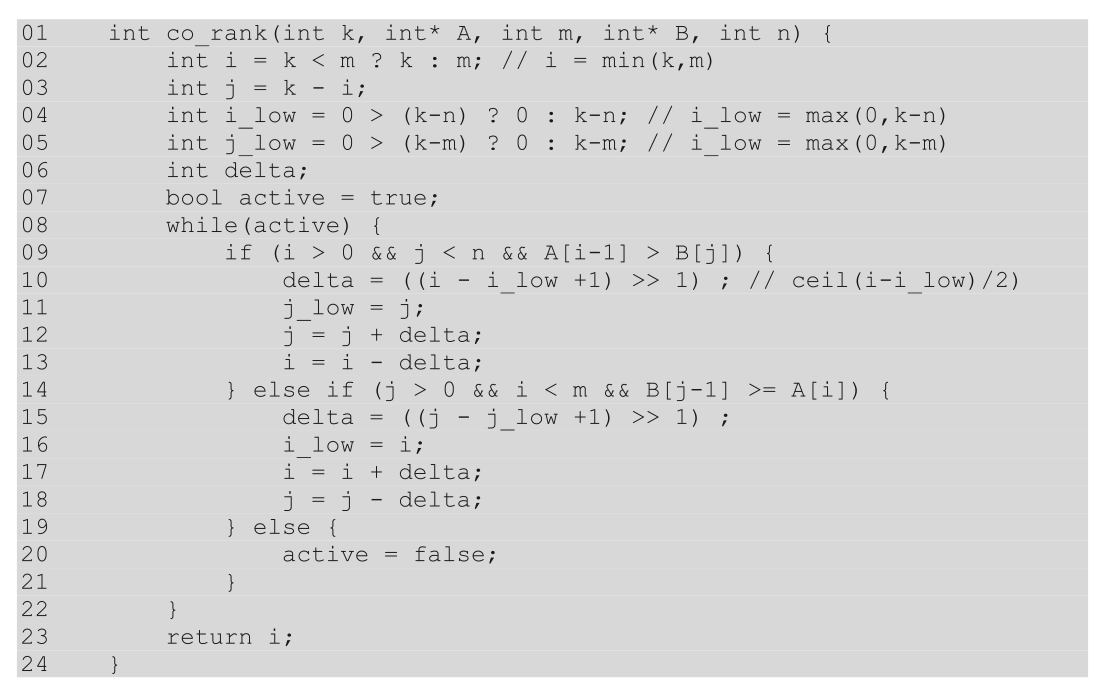
\includegraphics[width=0.9\textwidth]{figs/F12.5.png}
	\caption{\textit{设备查询机制的简单使用:curious.cpp }}
\end{figure}

\begin{figure}[H]
	\centering
	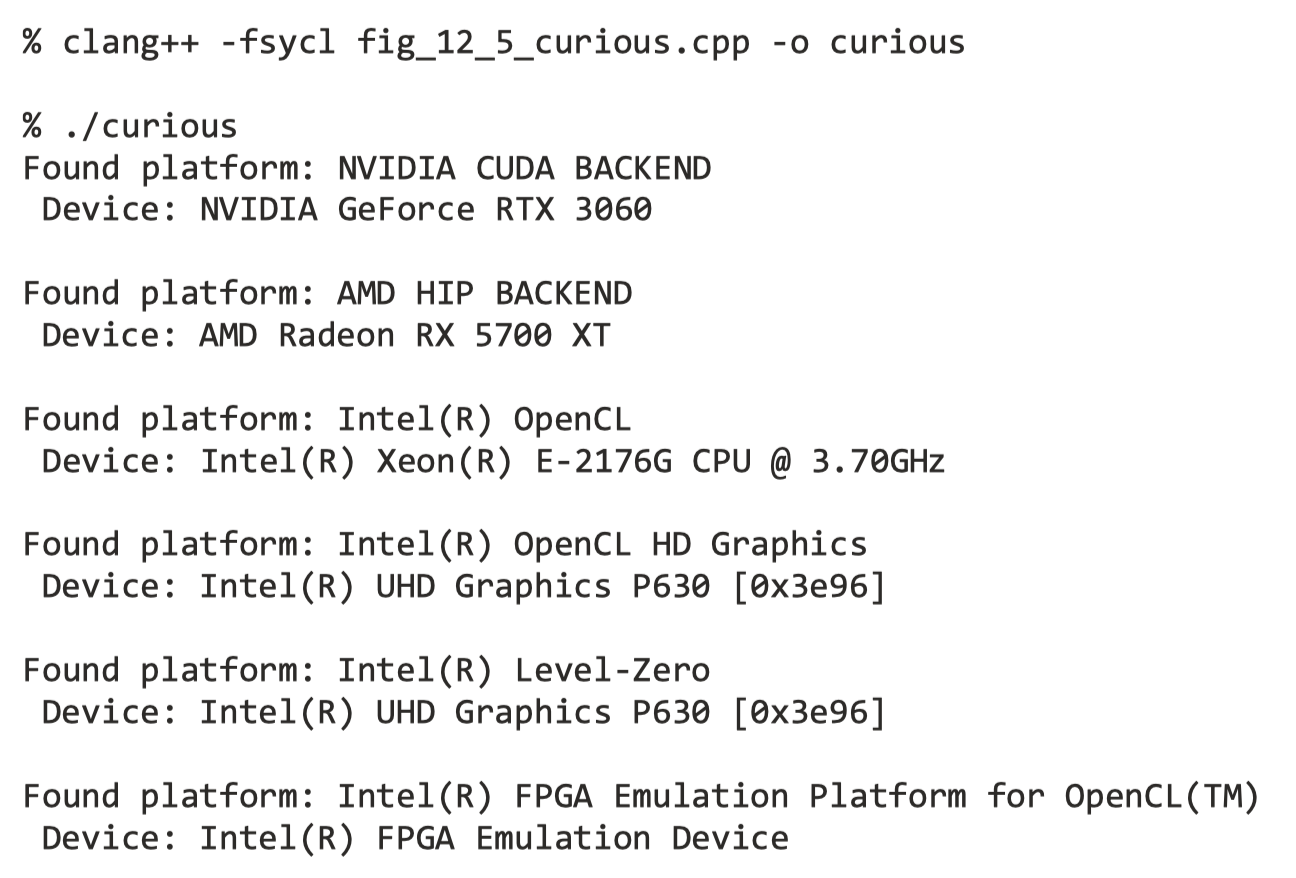
\includegraphics[width=0.9\textwidth]{figs/F12.6.png}
	\caption{\textit{curious.cpp的输出示例 }}
\end{figure}

\subsubsection{更好奇:详细的枚举代码}
\begin{figure}[H]
	\centering
	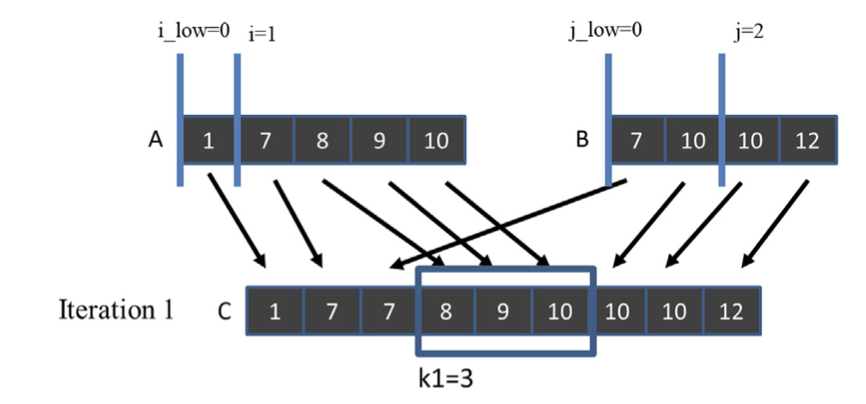
\includegraphics[width=0.9\textwidth]{figs/F12.7.png}
	\caption{\textit{设备查询机制的更详细使用:verycurious.cpp(显示的子集) }}
\end{figure}

我们提供了一个程序,我们将其命名为verycurious.cpp(图12-7),来说明使用get\_info 可以获得的一些详细信息。 
我们再次发现自己编写这样的代码来帮助开发或调试程序。

现在我们已经展示了如何访问信息,我们将讨论在应用程序中查询和操作最重要的信息字段。

\subsubsection{非常好奇:get\_info 加上 has()}
has() 接口允许程序使用图 12-3 中列出的Aspect直接测试某个功能。 
简单的用法如图 12-7 所示,更多内容请参见 GitHub 书中完整的verycurious.cpp 源代码。
 verycurious.cpp 程序有助于查看系统上设备的详细信息。

\subsection{设备信息描述符}
本章前面使用的“好奇”和“非常好奇”程序示例利用流行的 SYCL 设备类成员函数
(即 is\_cpu、is\_gpu、is\_accelerator、get\_info、has)。 
这些成员函数记录在 SYCL 规范中标题为“SYCL 设备类的成员函数”的表中。

“好奇”的程序示例还使用 get\_info 成员函数查询信息。 所有 SYCL 设备都必须支持一组查询。 
SYCL 规范中标题为“设备信息描述符”的表中描述了此类项目的完整列表。

\subsection{设备特定的Kernel信息描述符}
与平台和设备一样,我们可以使用 get\_info 函数查询有关Kernel的信息。 
此类信息(例如,支持的Work-Groups大小、首选Work-Groups大小、每个工作项所需的私有内存量)可能是特定于设备的,
因此Kernel类的 get\_info 成员函数接受设备作为参数 。

\subsection{细节:“正确性”的细节}
我们将细节分为有关必要条件(正确性)的信息和对调整有用但对正确性不是必需的信息。

\begin{figure}[H]
	\centering
	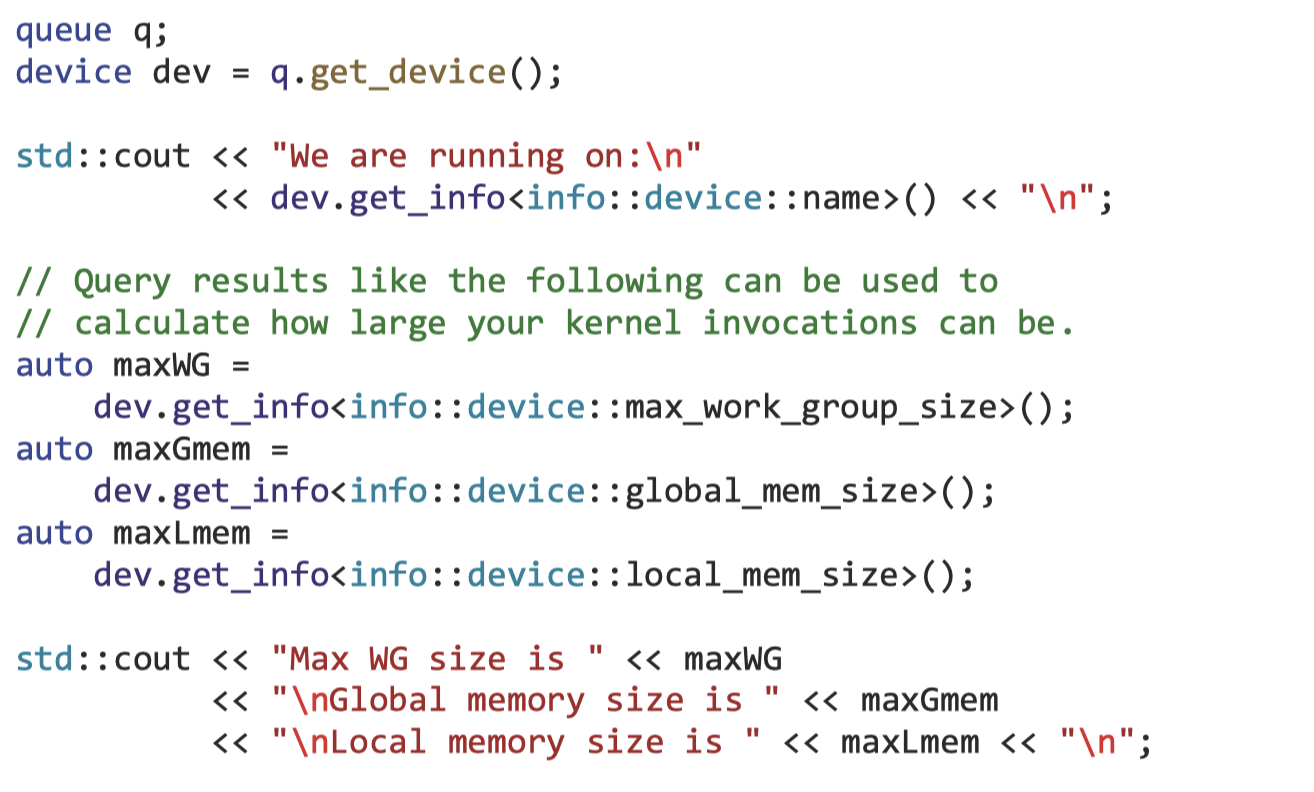
\includegraphics[width=0.9\textwidth]{figs/F12.8.png}
	\caption{\textit{获取可用于塑造Kernel的参数 }}
\end{figure}

\begin{remark}
	提交违反必需条件(例如 sub\_group\_sizes)的Kernel将生成运行时错误。
\end{remark}

在第一个正确性类别中,我们将列举Kernel正确启动应满足的条件。 不遵守这些设备限制将导致程序失败。 
图 12-8 显示了我们如何获取其中一些参数,使这些值可用于主机代码和Kernel代码(通过 lambda 捕获)。 
我们可以修改我们的代码以利用这些信息; 例如,它可以指导我们的代码确定缓冲区大小或Work-Groups大小。

\subsubsection{设备查询}
device\_type:cpu、gpu、加速器、自定义
\footnote{本书不讨论自定义设备(不要将“自定义设备”与“自定义设备选择器”混淆)。
如果我们发现自己使用自定义类型对标识自己的设备进行编程,我们将需要研究该设备的文档以了解更多信息。
说得不那么委婉:定制设备并不常见且很奇怪,
所以我们不打算谈论它们——我们故意忽略了它们可能对我们讨论的某些功能施加的限制。}
、自动、全部。 
这些最常通过 is\_cpu、is\_gpu() 等进行测试(参见图 12-7):

max\_work\_item\_sizes:nd\_range 的Work-Groups的每个维度中允许的最大工作项数。 最小值为 (1, 1, 1)。

max\_work\_group\_size:在单个计算单元上执行Kernel的Work-Groups中允许的最大工作项数。 最小值为 1。

global\_mem\_size:全局内存的大小(以字节为单位)。

local\_mem\_size:本地内存的大小(以字节为单位)。 最小大小为 32 K。

max\_compute\_units:指示设备上可用的并行量 - 实现定义的,请小心解释!

sub\_group\_sizes:返回设备支持的子组大小集。

请注意,还有更多特性被编码为Aspect(参见图 12-3),例如 USM 功能。

\begin{remark}[我们强烈建议避免在程序逻辑中MAX\_COMPUTE\_UNITS]
我们发现,应该避免查询最大数量的计算单元,部分原因是定义不够清晰,无法在代码优化中发挥作用。
大多数程序应该表达它们的并行性,并让运行时将其映射到可用的并行性上,而不是使用 max\_compute\_units。
依靠max\_compute\_units的正确性只有在使用特定于实现和设备的信息进行增强时才有意义。
专家可能会这样做,但大多数开发人员不会也不需要这样做!在这种情况下,让运行时完成它的工作!
\end{remark}

\subsubsection{Kernel查询}
执行这些Kernel查询需要第 10 章“Kernel捆绑中的Kernel”下讨论的机制:

work\_group\_size:返回可用于在特定设备上执行Kernel的最大Work-Groups大小

compile\_work\_group\_size:返回Kernel指定的Work-Groups大小(如果适用); 否则返回 (0, 0, 0)

compile\_sub\_group\_size:返回Kernel指定的子组大小(如果适用); 否则返回 0

compile\_num\_sub\_groups:返回Kernel指定的子组数量(如果适用); 否则返回 0

max\_sub\_group\_size:返回使用指定Work-Groups大小启动的Kernel的最大子组大小

max\_num\_sub\_groups:返回Kernel的最大子组数

\subsection{具体内容:“调整/优化”的具体内容}
有一些额外的参数可以被视为我们Kernel的微调参数。 
可以忽略这些,而不会危及程序的正确性。 这些使我们的Kernel能够真正利用硬件的细节来提高性能。

\begin{remark}
	在优化缓存(如果存在)时,注意这些查询的结果会有所帮助。
\end{remark}

\subsubsection{设备查询}
global\_mem\_cache\_line\_size:全局内存缓存行的大小(以字节为单位)。

global\_mem\_cache\_size:全局内存缓存的大小(以字节为单位)。 

local\_mem\_type:支持的本地内存类型。 这可以是 info::local\_mem\_type::local 表示特化本地内存存储,
例如 SRAM 或 info::local\_mem\_type::global。 
后一种类型意味着本地内存只是作为全局内存之上的抽象实现,可能没有性能提升。

\subsubsection{Kernel查询}
Preferred\_work\_group\_size:在特定设备上执行Kernel的首选Work-Groups大小。

Preferred\_work\_group\_size\_multiple:Work-Groups大小应是此值 (preferred\_work\_group\_size\_multiple) 的倍数,以便在特定设备上执行Kernel以获得最佳性能。 
该值不得大于work\_group\_size。

\subsection{运行时与编译时属性}
实现可能提供编译时常量/宏或其他功能,但它们不是标准的,因此我们不鼓励使用它们,也不会在本书中讨论它们。 
本章中描述的查询是通过运行时 API (get\_info) 执行的,因此直到运行时才知道结果。 
在下一节中,我们将讨论如何使用属性来控制Kernel的编译方式。 
除了属性之外,SYCL 标准仅提倡使用运行时信息,但有一个相当深奥的例外。 
SYCL 确实提供了应用程序可用于在编译时查询Aspect的两个特征。 
这些特征特化用于帮助避免为任何设备不支持的设备功能实例化模板化Kernel。 
这是一个非常高级且很少使用的功能,我们在本书中不会详细说明。 
SYCL 标准在“设备Aspect”部分末尾有一个示例,
该示例展示了为此目的使用any\_device\_has\_v<aspect> 和all\_devices\_have\_v<aspect>。 
该标准还定义了“特化常量”,我们在本书中不讨论它们,因为它们通常用于非常高级的目标开发,例如在库中。 
结语中“编译时属性”下讨论了实验性编译时属性扩展。

\subsection{Kernel特化}
我们可以通过针对不同用途使用不同的Kernel来特化我们的Kernel,
并根据我们目标设备的各个Aspect(参见图 12-3)选择适当的Kernel。 
当然,我们可以显式编写特化的Kernel并使用 C++ 模板来提供帮助。 
我们可以通过使用 SYCL 属性(图 12-9)和Aspect(图 12-3)来通知编译器我们希望Kernel使用特定功能。

\begin{figure}[H]
	\centering
	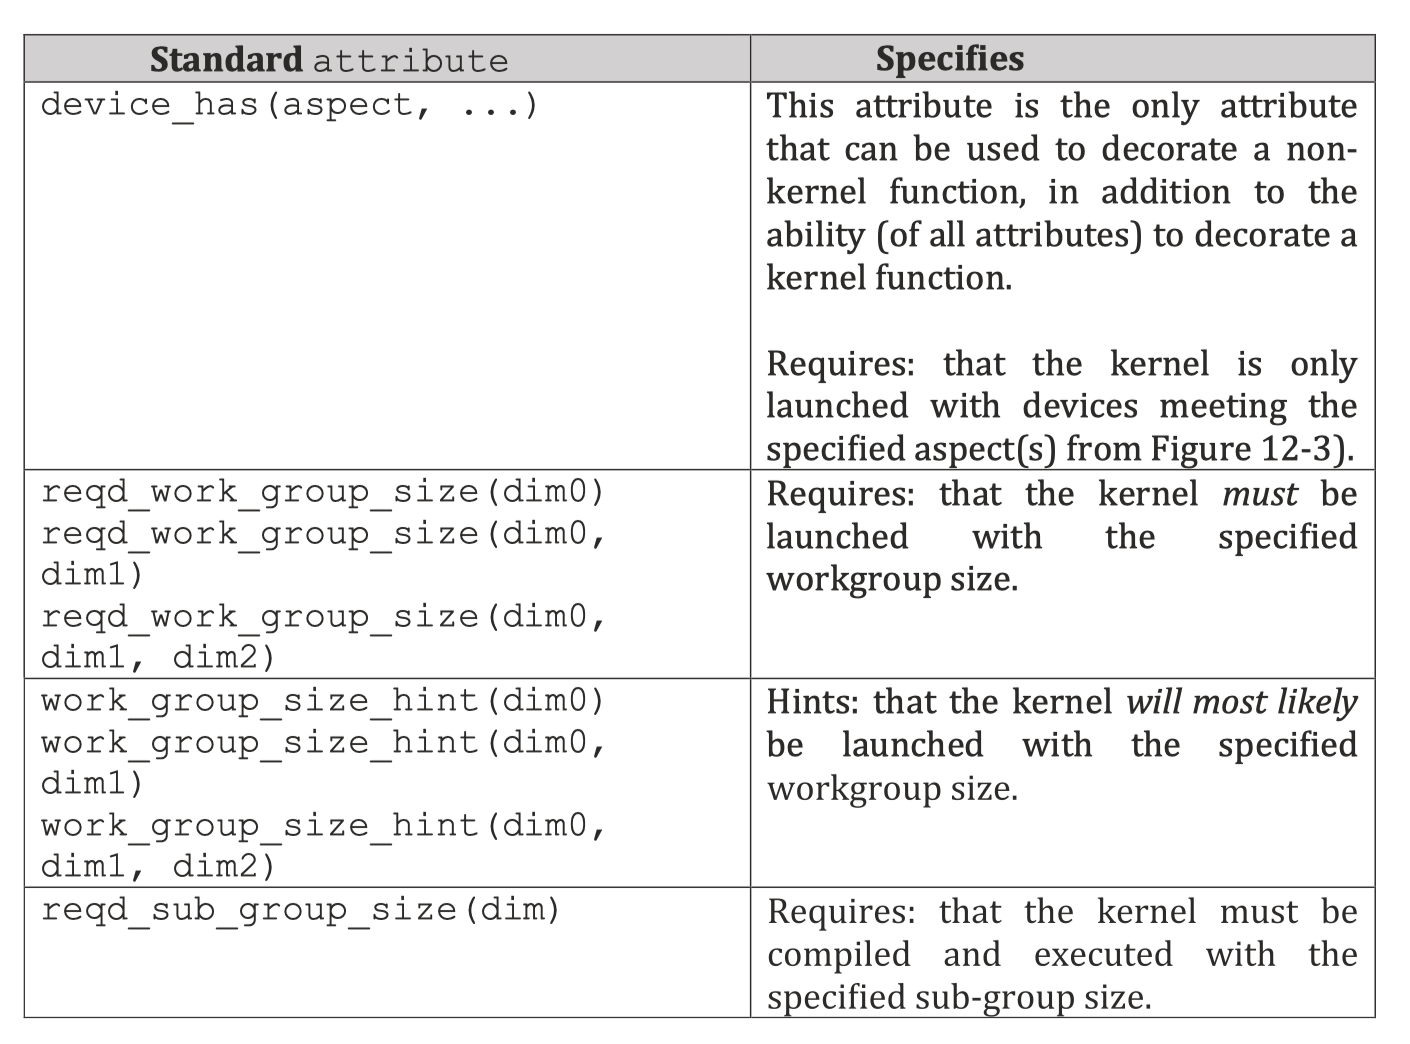
\includegraphics[width=0.9\textwidth]{figs/F12.9.png}
	\caption{\textit{由 SYCL 标准定义的属性(未弃用) }}
\end{figure}

\begin{figure}[H]
	\centering
	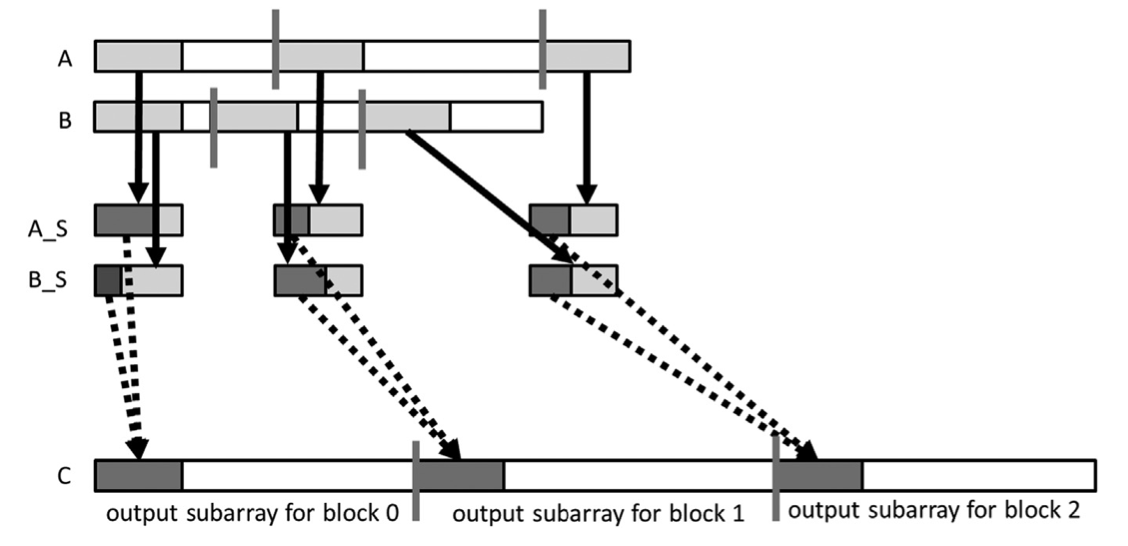
\includegraphics[width=0.9\textwidth]{figs/F12.10.png}
	\caption{\textit{借助属性显式Kernel特化 }}
\end{figure}

例如,reqd\_work\_group\_size 属性(图 12-9)可用于要求Kernel的特定Work-Groups大小,
而 device\_has 属性可用于要求Kernel的特定设备Aspect。

使用属性有两个作用:

\begin{enumerate}
	\item 如果Kernel提交到不具有所列Aspect之一的设备,则Kernel将引发异常。

	\item 如果Kernel(或其调用的任何函数)使用与属性中未列出的Aspect关联的可选功能(例如,fp16),
	编译器将发出诊断信息。
\end{enumerate}

第一个有助于防止应用程序在可能失败的情况下继续运行,第二个有助于在编译时捕获错误。 
由于这些原因,使用属性会很有帮助。

图 12-10 提供了一个示例,该示例使用运行时逻辑在两个代码序列之间进行选择,并使用属性来特化其中一个Kernel。

\subsection{总结}
最可移植的程序将查询系统中可用的设备,并根据运行时信息调整其行为。 
本章打开了获取丰富信息的大门,这些信息可用于允许对我们的代码进行此类定制以适应运行时存在的硬件。 
我们还讨论了特化Kernel的各种方法,以便当我们认为投资值得时,它们可以更紧密地适应特定的设备类型。 
这些为我们提供了必要的工具来平衡可移植性和性能以满足我们的需求,所有这些都在使用 C++ 和 SYCL 的范围内。

通过对我们的应用程序进行参数化以适应硬件的特性,我们的程序可以在功能上更加便携,在性能上更加便携,并且更加面向未来。 
我们还可以测试当前的硬件是否在我们在程序设计中所做的任何假设的范围内,并且当发现硬件超出我们的假设范围时发出警告或中止。